Since the 1970s \parencite{article14}, the decade in which the microprocessor era started, the overall performance of a processor has increased \parencite{inproceedings4}. This goal was achieved by several points, including ``\textit{sophisticated process technology, innovative architecture or micro-architecture}'' \parencite[see][Chapter 1, p2]{inproceedings4}. In fact, increasing the clock speed of a single core processor, like Moore's Law predicted \parencite{article14}, was usually reached by increasing the number of transistors on the chip \parencite{article14}. However, this go along side with the increase in complexity \parencite[see][Pollack’s rule]{article14}, which mean, that doubling the logic of a processor result in a performance boost of only 40\% \parencite[see][Chapter 2]{article14}.

Another huge problem chip manufacturers have to deal with is leakage power \parencite[see][Chapter 2, p3]{inproceedings4}, because the ``\textit{transistor leakage current increases as the chip size shrinks}'' \parencite[see][p2]{article14} [see Chart \ref{fig:leackagePer}]. An increase of leakage current of the transistors also result in a increase of the die's temperature \parencite{inproceedings4} along side the total power consumption as well.
\begin{figure}[h!]
	\centering
	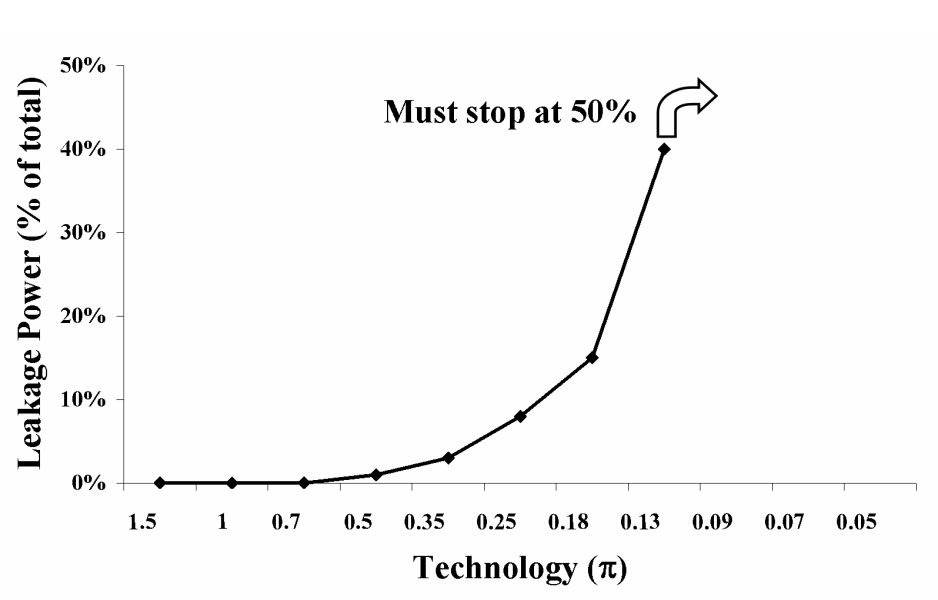
\includegraphics[scale=0.25]{leackage-power_vs_process-technology.png}
	\caption{
		Leakage Power (\% of total) vs. process technology \parencite{inproceedings4}
	}
	\label{fig:leackagePer}
\end{figure}

Furthermore, a increase of the processor clock frequency to speed up the performance is only available to a suffisticating limit of 4GHz \parencite{article14}. After this frequency threshold, also known as reaching the power wall, the ``\textit{power dissipation}'' \parencite[see][p2]{article14} increases again.

Facing these types of problems such as ``\textit{chip fabrication costs, fault tolerance, power efficiency, heat dissipation}'' \parencite[see][p3]{article14} along side with increasing processor performance, the only possible solution chip manufacturers and companies could offer was parallelism. 

\newpage

\section{Basic Concept}

Parallelism for processing is not something new. But due to the fact that real thread level parallelism [see Chapter \ref{subchap:threadLevelParallelism}] was only available after dual or multi-core processors were invented in 2005 \parencite{internet6}, the topic itself and efficient software implementations are still treated in scientific work \parencite{book3} \parencite{article2}.

\begin{figure}[h!]
	\centering
	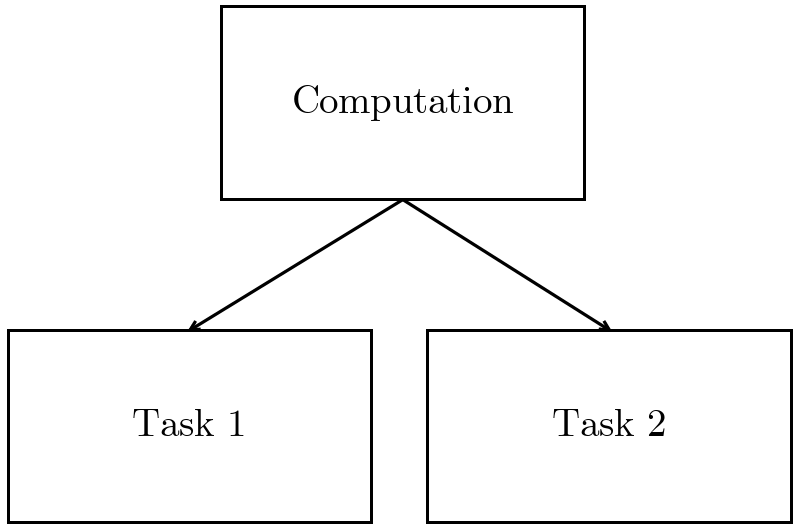
\includegraphics[scale=0.3]{basic-parallelism.png}
	\caption{
		The basic concept of a simple concurrency computation.
	}
	\label{fig:basicPara}
\end{figure}

In general, parallelism for programming means to split up a task or a computation into several sub tasks [e.g. Figure \ref{fig:basicPara}] or results, to decrease the execution time. Depending on the problem itself, these separated tasks can be independent or connected [see Chapter \ref{chap:parallelPrinciples}]. If we want to talk about the general concept of parallelism, we have to take a closer look to some mathematical laws, which try to describe the availability to parallel task execution and their limits.

\subsection{Amdahl's Law}

The first one, which quantifies parallelism, is called Amdahl's Law \parencite{inbook1}. During the publication period of Amdahl's paper \parencite{book6}, critics claimed ``\textit{that the organization of a single computer has reached its limits and that
truly significant advances can be made only by interconnection of a multiplicity of computers}” \parencite[see][p80]{inbook1}. Of course this can be transferred on single and multi-core processors or even on multi threading \parencite[see][Chapter 1.3, p2]{phdthesis1}, but in fact, like Amdahl claimed too, addressing hardware \parencite{inbook1}, and nowadays switching context time was not considered in this case.

Amdahl's Law wants ``\textit{to provide an upper limit on speedup}'' \parencite[see][p81]{inbook1} in general to point out that there is a overhead \parencite{inbook1}, which can not pe implemented in parallel, but at the same time, ``\textit{apart from the sequential fraction, the remaining computations are perfectly parallelizable}'' \parencite[see][p81]{inbook1}.

\newpage

\begin{figure}[h!]
	\centering
	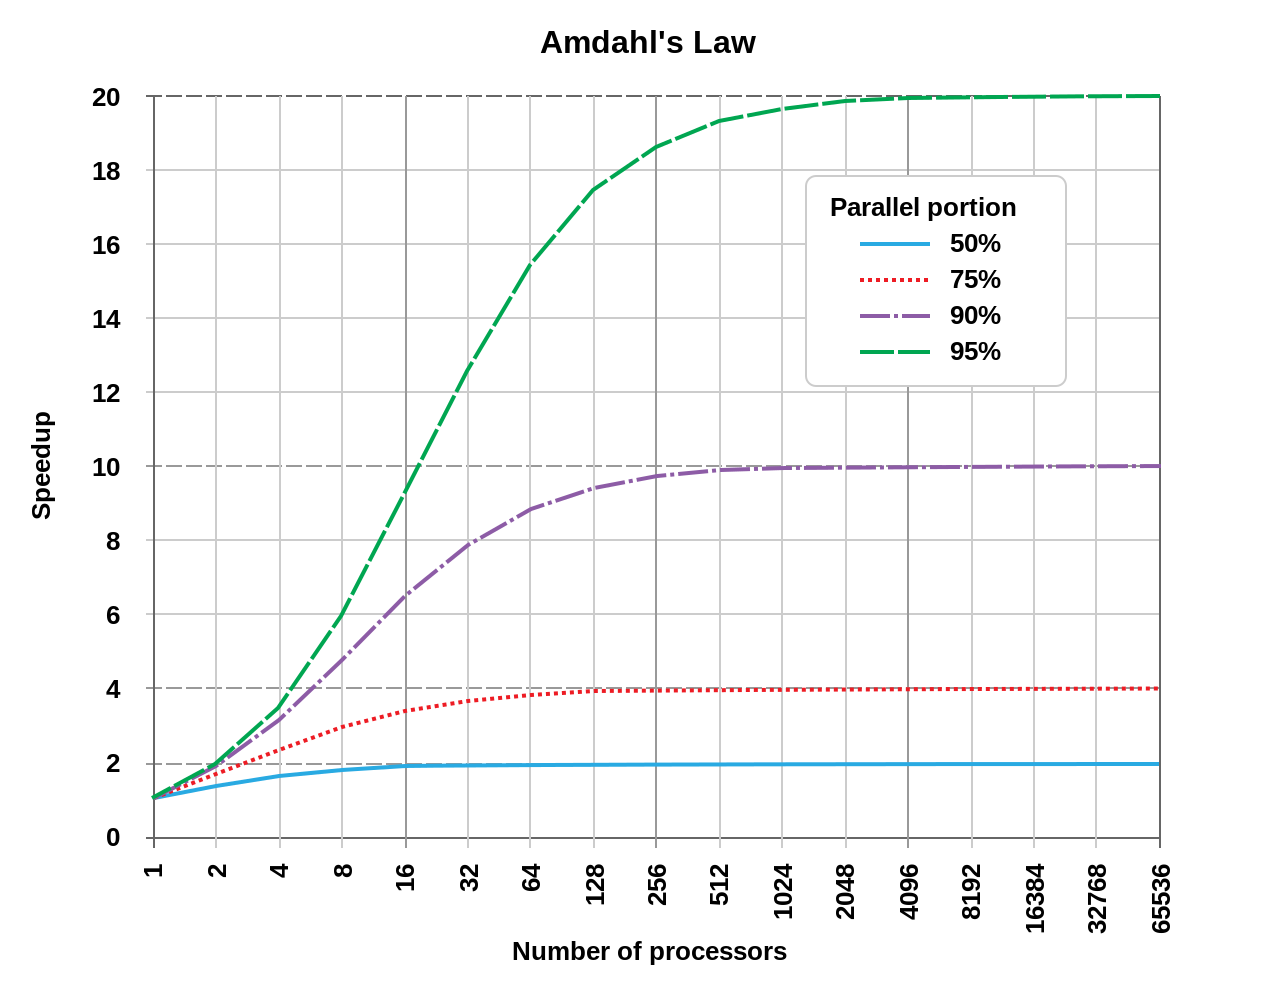
\includegraphics[scale=0.95]{amdahls-law.png}
	\caption{
		The limited speed-up of a program, which can be parallelized, depending on the number of parallel executions \parencite{image1} \parencite[similar to][p4]{phdthesis1}.
	}
	\label{fig:admLaw}
\end{figure}

\noindent So regarding to Amdahl's Law, there has to be an upper limit of parallelism, due to the fact, that some sequential fractions still exists. In order to be able to describe this relationship, the time required to perform a calculation at once is related to the total time in parallel execution:

``\textit{Let t\textsubscript{1} be the time taken by one processor solving a computational problem and t\textsubscript{p} be the time taken by p processors solving the same problem. Finally let us denote the supposed inherently sequential fraction of instructions by f. Then, according to Amdahl, t\textsubscript{p} = t\textsubscript{1}(f+(1-f)/p) and the speedup obtainable by p processors can be expressed as}'' \parencite[see][p81]{inbook1}:

\begin{equation} \label{formula:amd}
	s = \frac{t_1}{t_p} = \frac{1}{f + (1 - f) / p}
\end{equation}
\\[2pt]
For example, a program which contains 90\% of parallelizable code [see Figure \ref{fig:admLaw}] reaches his speed up limit at around 512 cores [formula  \ref{formula:amdLimes}]; in this case we substitute f= 0.2/2. After that number of processor cores, an significant speed up increase is not noticeable anymore . 

\begin{equation} \label{formula:amdLimes}
	\lim_{p \to \infty f \to 0.1} \left( \frac{t_1}{t_p} \right) = \lim_{p \to \infty} \left( \frac{1}{0.1 + (1 - 0.1) / p} \right) = 10
\end{equation}
\\[2pt]
Many other authors tried to claim that this upper limit of speed up, both in theory and practice, is not the final end. To proof that, only to mention a few , they took into account the ``\textit{energy per instruction (EPI)}" \parencite[Annavaram et al. in][Chapter 3,  p81]{inbook1}, a case study depending on ``\textit{asymmetric (or heterogeneous) chip multiprocessor architectures}'' \parencite[Kumar et al. in][Chapter 3,  p81]{inbook1} or even considering ``\textit{disk arrays to reduce input-output requirements}'' \parencite[Patterson et al. in][Chapter 3,  p81]{inbook1}.

\newpage

\subsection{Gustafson’s Law's}

Due to the fact that Gustafson’s Law's is based on ``\textit{the same concepts as the
bases of Amdahl’s law, it is more a variant, rather than a refutation}'' \parencite[see][p81]{inbook1}. But in fact, it is another mathematical consideration, which offers, in comparison to Amdahl's Law, no upper speed up limit regarding parallelism. Related to Gustafson, the time a single core processor needs solving the same computational problem on the sequential would be \textit{ft\textsubscript{p}}, and on the parallelizable part \textit{(1-f)pt\textsubscript{p}}. Therefore, the total amount of achievable speed up by p processors can thus be calculated

\begin{equation} \label{formula:gustLaw}
	s = \frac{t_1}{t_p} = \frac{ft_p + (1 - f)pt_p}{t_p} = f + (1 - f)p
\end{equation}
\\[2pt]
using the formula \ref{formula:gustLaw} above. In this case, ``\textit{f is the same “inherently sequential” fraction of instructions as in the case of Amdahl’s law}'' \parencite[see][p81]{inbook1}. In addition to that, he doesn't take the ``\textit{sequential input-output requirements proportional to input and output sizes into account}'' \parencite[see][p81]{inbook1}.

\begin{figure}[h!]
	\centering
	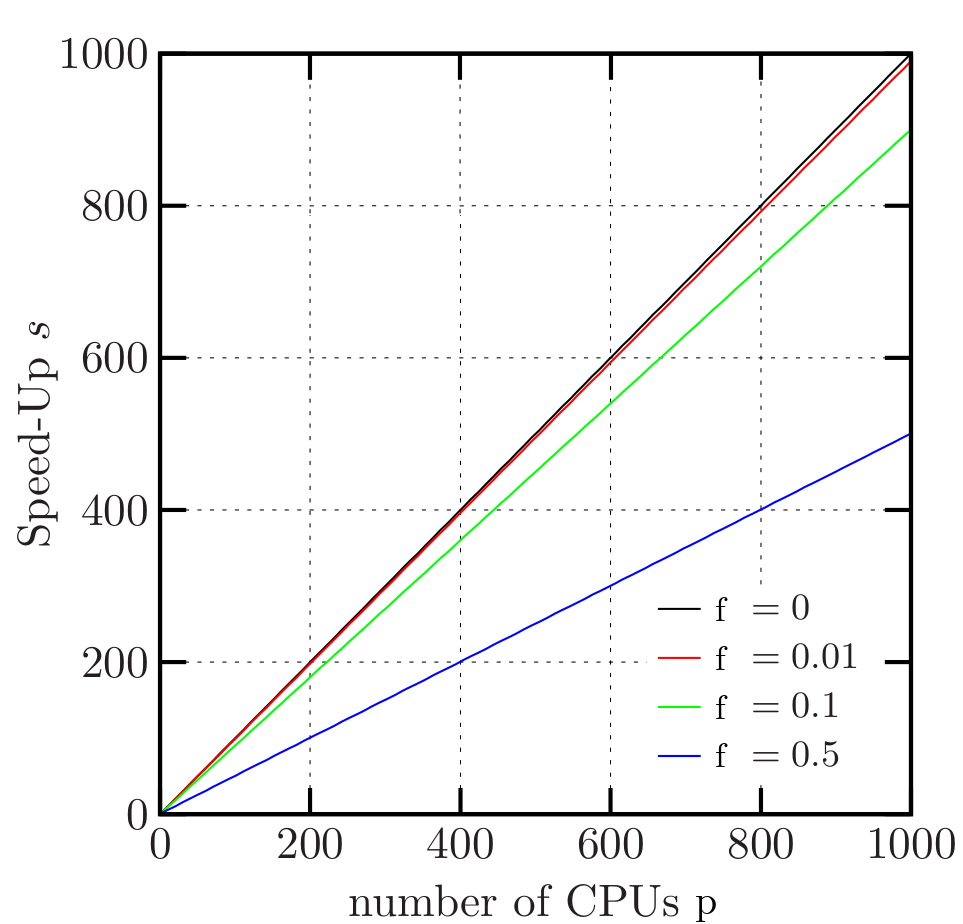
\includegraphics[scale=0.28]{gustafssons-law.png}
	\caption{
		Gustafson’s Law. In contrast to Amdahl we now have no upper limit to the speed up. \textit{f} only determines the slope of the speed-up \parencite{article19}.
	}
	\label{fig:gustLaw}
\end{figure}

Regarding to \parencite{inbook1}, neither Amdahl's or Gustafson’s Law are suitable to quantify parallelism in theory and practice, because both don't take into account, that ``\textit{sequential fractions of computations have negligible effect on speedup if the growth rate of the parallelizable fraction is higher than that of the sequential fraction}'' \parencite[see][Chapter 7, p88]{inbook1}.

Furthermore, \parencite{inbook1} point out, that no simple formula governing parallelism exists. Both laws are more of an attempt to describe experimental results, and therefore understood rather as a draft rule of thumb as a law.

\newpage

\subsection{Principles of Parallel Computing}\label{chap:parallelPrinciples}

Despite trying to quantify the ability to parallelism task processing, it is also important to keep in mind the basic aim of parallelism to mention a ``\textit{design for concurrency}'' \parencite[see][p4]{article6}. First of all, reducing the execution time is one of the most important objective in concurrency to make applications more \textbf{efficient}. Computations, and even tasks, are getting more and more complicated \parencite{internet2}, not only in the application field of scientific researches. Today's software applications require sophisticated hardware like multi-core processors, to offer a suitable user experience, for example in gaming (e.g VR), augmented reality in automation (e.g. AR) or for IoT [see Chapter \ref{chap:introduction}] devices.

\begin{figure}[h!]
	\centering
	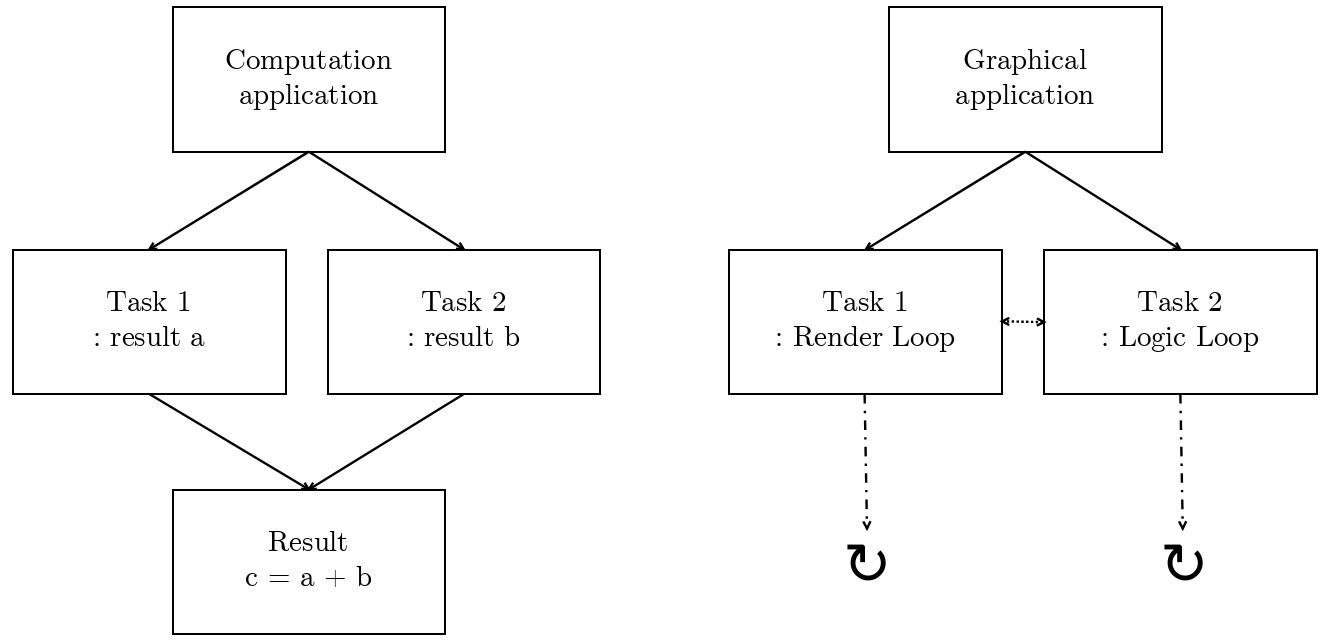
\includegraphics[scale=0.32]{comparison-comp-indep-par-depnd-par.png}
	\caption{
		Comparison of independent and dependent tasks in a general concurrency application.
	}
	\label{fig:compIndeDepConcurr}
\end{figure}

In case of software parallelism, which is the main objective of this chapter, we have to distinguish between tasks, which are independent and tasks, which are connected (called dependent). It depends largely on the application itself: e.g. for example, a numerical calculation [see Chapter \ref{chap:mathComp}] can be easily subdivided into sub tasks to speed up the computation, whereas a graphical application needs a logical loop and a render loop, both independently in different tasks [see Fig. \ref{fig:compIndeDepConcurr}]; a data exchange usually takes place via a shared memory [more on this in Chapter \ref{chap:parallelCompArch}]. As already suggested in Chapter \ref{fig:basicPara}, our work will be limited to the division of numerical or generic mathematical calculations. 

In addition to that, multi-core software applications offers also the opportunity, to provide low power systems, because \textbf{power consumption} results from performance and clock frequency \parencite[see][Fig. 3, p4]{article14}, along side instructions per core (IPC) \parencite{inproceedings4} [further inf. in Chapter \ref{chap:parallelprg}].

\newpage

\begin{figure}[h!]
	\centering
	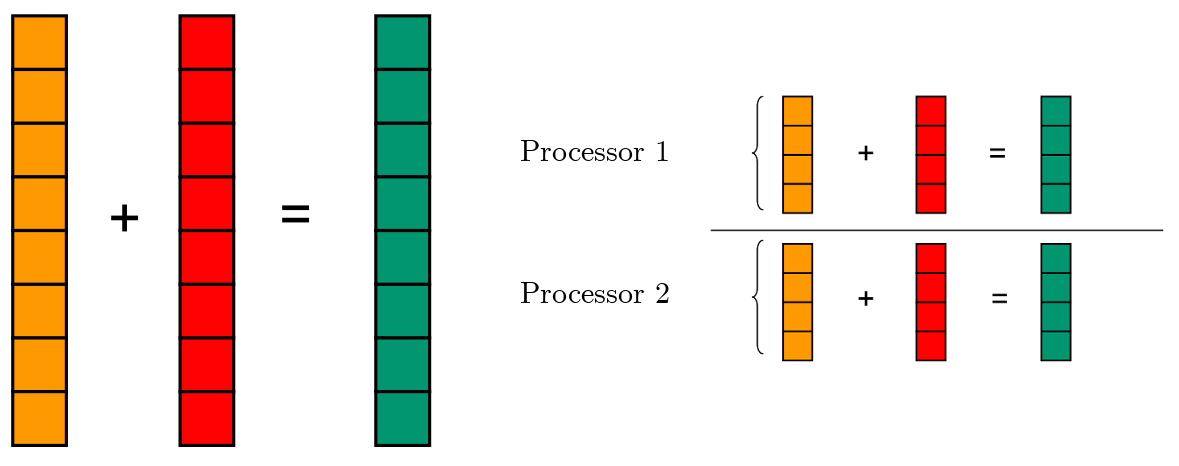
\includegraphics[scale=0.25]{array-split-parallelism.png}
	\caption{
		Adding to arrays of integers for speed up in concurrency \parencite[see][p3]{internet2}.
	}
	\label{fig:arraySplit}
\end{figure}

\noindent Furthermore, to guarantee \textbf{flexibility} for both, the software application and hardware platform, multi-core systems and concurrency is the way to go to fit customers and companies claims. This can easily be proofed due to the fact that today's hard- and software manufacturers always try to provide generalized solutions.   

It can not be denied that as the degree of parallelism increases, the complexity of the application including the hardware realization also increases \parencite{article14} \parencite{article6}. A basic principle and design pattern of parallel computing is therefore to ensure maximum efficiency through parallelism while reducing complexity. A usual rule can be transferred on this topic: ensure \textbf{simplicity}.

Regarding to Figure \ref{fig:compIndeDepConcurr} and Chapter \ref{chap:mathComp}, the best way to implement and computation concurrent is to guarantee that the sub tasks can work independent from each other. This has a major effect on the performance and complexity of the software implementation: ``massively parallel vs. embarrassingly serial'' \parencite[see][p15]{article6}, alongside the ability to take less attention on control issues such as task orders, synchronization, (shared) memory access or even task communication \parencite{internet1}. In fact, complete concurrency is not possible, due to the fact that splitting a computation into sub tasks requires at least on remaining worker task to collect and combine the sub task results. Anyway, \textbf{Independence} of sub tasks enables almost the best efficiency.\\

\noindent \textbf{Emphasises design}  \parencite[see][p5]{article6}: In summary, therefore, the following points should be seen as goals and thus as groundbreaking for the basic principles of parallelism:

\begin{enumerate}
	\item \underline{Efficiency}: 
	
	Concurrency in hard- and software to solve large problems in less amount of time to reduce execution time and power consumption.
		
	\item \underline{Flexibility}: 
	
	Environments will be more heterogeneous and the use in different application areas will be enabled.
	
	\item \underline{Simplicity}:
	
	Code for Parallel Computing will be more complicated, because synchronization or memory access have to be regulated. One reason more ``\textit{to strive for maintainable,
	understandable programs}'' \parencite[see][p6]{article6}. 
	
	\item \underline{Independence}:
	
	To ensure maximum efficiency, parallel computations should be independent.
\end{enumerate}

\newpage

\noindent These principles result in four different \textbf{design patterns} \parencite[see][p11 ff.]{article6} for parallel software applications:
\begin{itemize}
  \item \underline{Finding concurrency}: 
  
  This should be the main aim of all software applications today, set the case it makes sense.
    \item \underline{Algorithm structure}: 
  
  To ensure proper efficient, the implementation should be based on usual parallel programming models [see Chapter \ref{chap:parPrgModels}].
  
  \item \underline{Supporting structures}: 
  
  ``\textit{Useful idioms rather than unique implementations}'' \parencite[see][p25]{article6} like Loop Parallelism, Fork/Join, Shared Data or Shared Queue \parencite{article6}.
  
  \item \underline{Implementation Mechanism}: 
  
  Using programming languages which offer the opportunity to real parallel computing (e.g. C++, OpenMP \& Pthreads, MPI, OpenCL) \parencite{article6}.
  
\end{itemize}

\section{Definition of parallel mathematical computations}\label{chap:mathComp}

We talked about how to quantifying parallelism, above that also about the principles of parallel computing and the resulting design patterns for parallel computing. Now its time to take into account the necessary mathematical computations. Not all calculations are suitable for parallelism, so we have to work out properties for the quantification of possible numerical or mathematical methods. 

\begin{equation} \label{formula:scalarVec}
\vec{a} = \begin{bmatrix}
a_{0} \\
a_{1} \\
\vdots \\
a_{i} \\
\vdots \\
a_{N - 1} \\
\end{bmatrix} ,\quad \vec{b} = \begin{bmatrix}
b_{0} \\
b_{1} \\
\vdots \\
b_{i} \\
\vdots \\
b_{N - 1} \\
\end{bmatrix}
\end{equation}

The easiest way to do that is to take a look an two basic examples. The first one will be a simple scalar product of two \textit{N} dimensional vectors $\vec{a}$ and $\vec{b}$ [see formula \ref{formula:scalarVec}]. Both vectors have the same dimension \textit{N} and are not orthogonal to each other; otherwise the scalar product would be very simple to calculate and the result null, regardless of the dimension of the vectors. The scalar product of two N dimensional vectors are defined as

\begin{equation} \label{formula:scalarProdEasy}
	s = \vec{a} \cdot \vec{b} = a_0 \cdot b_0 + a_1 \cdot b_1 + \quad \cdots \quad + a_{N - 1} \cdot b_{N - 1}
\end{equation}

\noindent or more formally like

\begin{equation} \label{formula:scalarProd}
	s = \sum_{i=0}^{N - 1} a[i] \cdot b[i]
\end{equation}

\newpage

As mentioned in formula \ref{formula:scalarProdEasy}, theoretically any kind of scalar product can be easily calculated in parallel using \textit{N} processor cores or tasks. We even don't have to take care about accessing resources, because all tasks will use their one values depending on the index of the vectors. Only in the end, the final result has to be calculated including the sub results, which are returned from the different tasks.

But to keep it simple, we will only separate the given scalar product [see formula \ref{formula:scalarProd}] into to different tasks. A synonymous representation would be the following:

\begin{align} \label{formula:scalarProdSeq}
	\begin{aligned}
		s &= \sum_{i = 0}^{N / 2 - 1} \left(a[i] \cdot b[i]\right) + \sum_{i = N / 2}^{N - 1} \left(a[i] \cdot b[i]\right)
		\\ &=  \underbrace{\sum_{i = 0}^{N / 2 - 1} \left(a_{local}[i] \cdot b_{local}[i]\right)}_\text{p\textsubscript{0}} \qquad \vertarrowbox{+}{process communication} \qquad \underbrace{\sum_{i = N / 2}^{N - 1} \left(a_{local}[i] \cdot b_{local}[i]\right)}_\text{p\textsubscript{1}}
	\end{aligned}
\end{align}

The important sign in formula \ref{formula:scalarProdSeq} is the ``+''. It seems inconspicuous, but in fact, this is the the one we have to take care about most. The ``+'' symbol indicates required ``communication between the processes'' \parencite[see][p]{internet2} p\textsubscript{0} and p\textsubscript{1}.

\newpage

\section{Parallel Computer Architecture}\label{chap:parallelCompArch}

The terminology of computer architecture was invented in 1960s by the designers of IBM System to describe the structure of a computer. Computer architect’s task is to write an suitable program code for the machine, keeping in mind every time this structure of computer, understanding all the factors like state-of-the-art technologies at each design level and changing those designs tradeoffs for their specific applications \parencite{article20}.

Parallel computing means the situation where tasks are separated into discrete parts that can be executed concurrently. Each part is diffused into a larger series of instructions which will be executed simultaneously on different CPU's or even in a pipeline [see Figure \ref{fig:parallelismPipe}]. These kind of parallel systems have to deal with the simultaneous use of multiple computer resources that can include either a single computer with multiple CPU's, or a number of computers connected by a network creating a parallel processing cluster or combination of both.

The crux of parallel processing are CPU's. Based on the number of instruction and data streams that can be processed simultaneously, computing systems are classified into four major categories based on Flynn’s Taxonomy \parencite{internet7}.

\begin{figure}[h!]
	\centering
	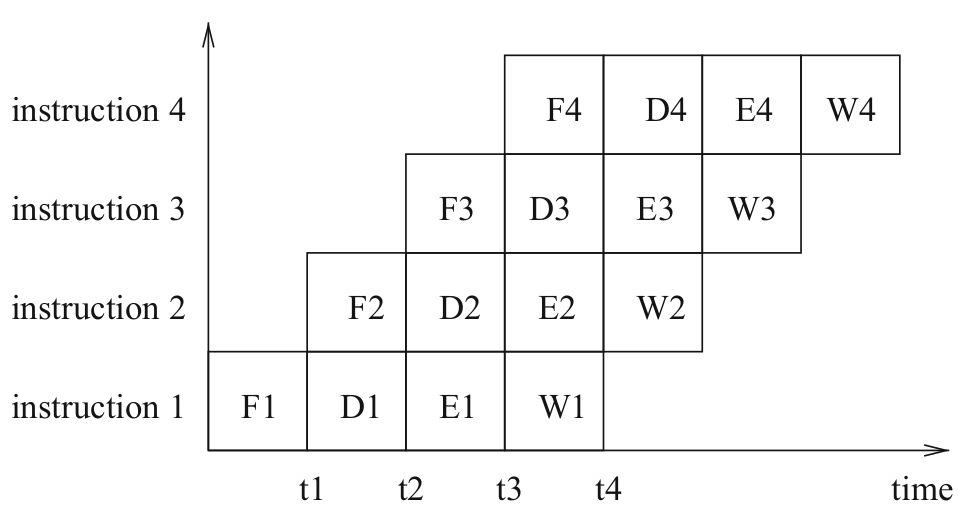
\includegraphics[scale=0.28]{parallelism-pipelining.png}
	\caption{
		Overlapping execution of four independent instructions by pipelining. The execution of each instruction is split into four stages: \textit{fetch (F)}, \textit{decode (D)}, \textit{execute (E)}, and \textit{write back (W)} \parencite[see][Fig. 2.1, p11]{book1}.
	}
	\label{fig:parallelismPipe}
\end{figure}

%...\parencite[see][p9]{book1} \\
%...examples of parallelism \parencite[see][p11]{book1} \\
%...links 1) \\
%...\parencite[see][p9 ff.]{book5}

\subsection{Flynn's Taxonomy of Parallel Architectures}

Flynn’s classification was first elaborated and proposed by Michael Flynn in 1966 and represents a scheme which is based on the notion of information stream. The term ‘stream’ defines a sequence or flow of either one of both existent types of information which flows and are operated into a processor: instructions or data. 

Instruction stream defines the sequence of instructions performed by CPU, as in the same time the data stream defines the data traffic exchanged between the memory and CPU.His taxonomy left aside the machine’s structure for classification of parallel computers and took over a whole new concept focusing on multiplicity of instructions and data streams observed by the CPU during execution.

\newpage

\noindent The major four categories are the followings [comp. to Fig. \ref{fig:flynnsTax}] \parencite{book1}:
\begin{enumerate}
	\item \underline{\textbf{SISD} (single-instruction, single-data) systems}:
	
		  It designs an sequential computer which exploits no parallelism in either the instruction stream nor data stream.  An SISD computing system  is a uniprocessor machine capable of single stream executions.
		  
	\item \underline{\textbf{SIMD} (single-instruction, multiple-data) systems}:
	
		  It designs a multiprocessor machine capable of executing a single instruction stream on multiple different data streams. Instructions can be executed sequentially, such as by pipe-lining,  or in parallel by multiple functional units.
		  
	\item \underline{\textbf{MISD} (multiple instruction streams, single data stream) systems}:
	
		  It designs a multiprocessor machine capable of executing different instructions streams on the same data stream.
	
	\item \underline{\textbf{MIMD} (multiple instruction streams, multiple data streams)  systems}:
	
		  It designs a multiprocessor machine capable of executing multiple instructions streams on multiple data streams. This architectures include multi-core superscalar processors and distributed systems. 	  
\end{enumerate}

\begin{figure}[h!]
	\centering
	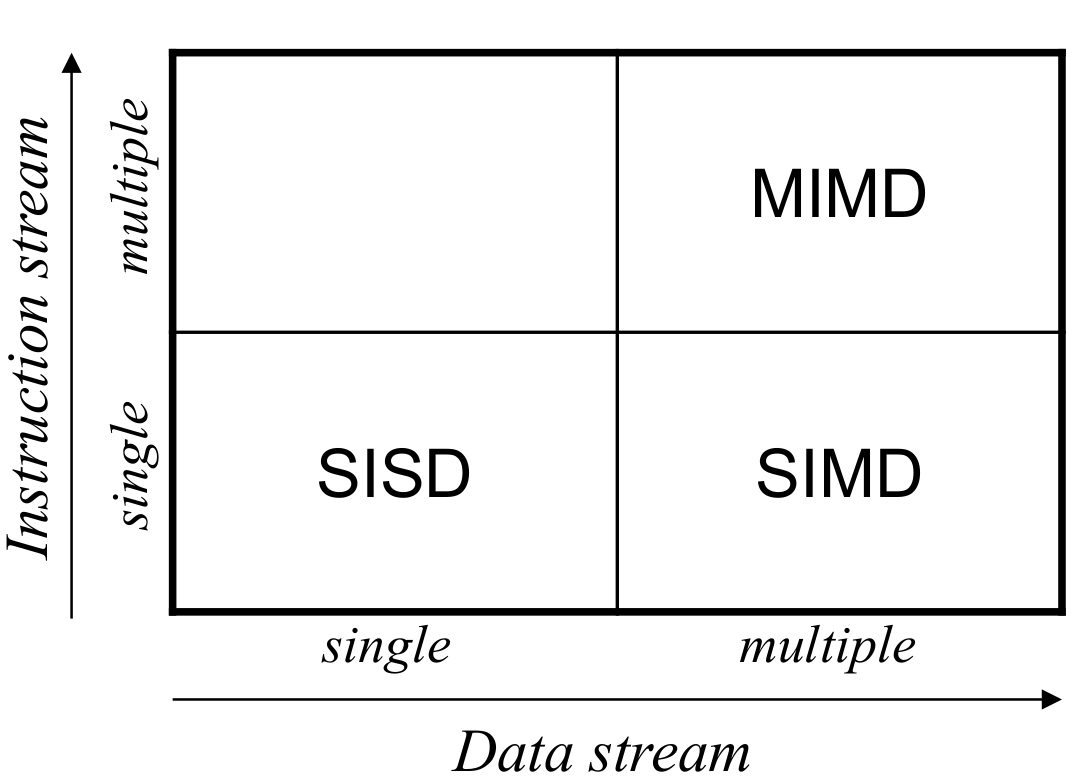
\includegraphics[scale=0.28]{flynns-taxonomy.png}
	\caption{
		Visualization of Flynn's Taxonomy \parencite[see][p5]{internet1}.
	}
	\label{fig:flynnsTax}
\end{figure}


\newpage

\subsection{Types of Parallelism}\label{subchap:typesOfParallelism}
<<<<<<< HEAD
=======
Parallel computing is used for multiple processing elements simultaneously to solve any type of problem, as it's already explained in [\ref{chap:parallelCompArch}].

The Parallel Computing is evolved from serial computing that attempts to emulate what has always been the state of affairs in natural World.
Advantages of Parallel Computing over Serial Computing:
\begin{enumerate}
			\item {It saves time and money as many resources working together will reduce the time and cut potential costs.}
			\item {It can be impractical to solve larger problems on Serial Computing.}
			\item {It can take advantage of non-local resources when the local resources are finite.}
			\item {Serial Computing ‘wastes’ the potential computing power, thus Parallel Computing makes better work of hardware.}
\end{enumerate}
Types of Parallelism:
\begin{enumerate}
	 \item {\textbf{Bit-level parallelism}: This form of parallelism computing have it's roots based in the concept of increasing the processor's size. The amount of instructons it's reduced that the system must execute in order to perform a task on large-sized data.}
	 \item {\textbf{Instruction-level parallelism}: This form of parallelism computing is designed for a processor to only address less than one instruction for each clock cycle phase. The instructions can be re-ordered and grouped which are later on executed concurrently without affecting the result of the program.}
	  \item {\textbf{Task/Thread parallelism}: This form of parallelism computing is designed to employ the subtasks fragments of a decompositioned task and then allocate the fragments subtasks for execution concurrently.} \parencite{book7}
\end{enumerate}   

\textbf{Thread-level parallelism} is the only way to execute independent programs or discrete parts of a single program,simultaneously, using different sources of execution, called threads.
>>>>>>> 49f3f2a7270328551412a189c1c8f9e54b00405c


\section{Parallel Programming Models}\label{chap:parPrgModels}

...

\newpage

\subsection{Classification of Parallel Programming Models}

\subsubsection{Process Interaction}

...\parencite[see][p4]{internet1}

\subsubsection{Problem decomposition}

...\parencite[see][p105 ff.]{book1}